\section{설계: 이벤트 집합 위의 합성곱}\label{sec:design}

이 장은 제안 커널 --- 이하 \emph{이벤트 커널}이라 부른다(제목의
무곱셈 희소 커널과 동일한 대상이다) --- 을 구현 절차가 아니라
원리의 체계로 서술한다.
출발점은 회수하려는 성질을 정확히 명제로 만드는 것이고(4.1절),
본체는 그 명제를 실제 성능으로 바꾸는 세 가지 설계
원리다(4.2--4.4절). 구현은 원리의 귀결로서 간략히
정리하고(4.5절), 마지막으로 이득의 구조를 1차 비용 모델로
추상화한다(4.6절). 그림~\ref{fig:concept}이 전체 대비를 요약한다.

\begin{figure}[htbp]
\centering
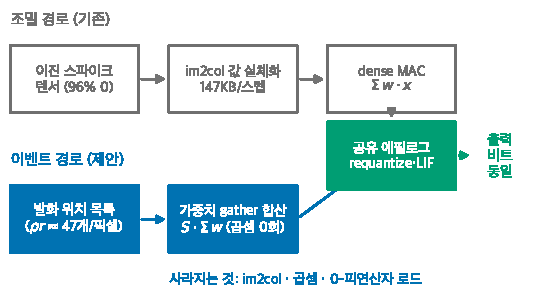
\includegraphics[width=0.98\linewidth]{figures/fig_concept.pdf}
\caption{조밀 경로(위)와 이벤트 경로(아래). 이진 활성에서는 값
실체화(im2col)와 곱셈이 원리적으로 불필요하다. 두 경로는 동일한
정수 에필로그를 공유하므로 출력이 비트 단위로 같다.}
\label{fig:concept}
\end{figure}

\subsection{대수적 기초와 의미 보존 계약}\label{sec:contract}

이 파이프라인의 모든 합성곱 입력은 이진이다: 첫 단은 인코더
출력 $\{0, 32{,}767\}$, 둘째 단은 LIF 스파이크 $\{0, S_1\}$이며,
제로 패딩은 비발화와 구별되지 않는다. 입력이 $\{0,S\}$이면 내적
길이 $r$의 곱셈-누산은 다음으로 붕괴한다:
\begin{equation}
\sum_{k=0}^{r-1} w_k\,x_k \;=\; S\cdot\!\!\sum_{k\in\mathcal{E}}\!w_k,
\qquad \mathcal{E}=\{k : x_k\neq0\}.
\label{eq:collapse}
\end{equation}
집합 $\mathcal{E}$가 바로 \emph{이벤트 집합}이다. 우변은 세 가지
이유로 좌변과 비트 단위로 같다. (i) 가중치 합은 int32에서 넘치지
않는다($|\sum w|\le r\cdot\max|w| = 1{,}152\times508 = 585{,}216 \ll
2^{31}$). (ii) $S$와의 곱과 바이어스 가산은 int64로 수행하므로
dense 경로의 64비트 누산과 같은 값이다. (iii) 정수 덧셈은
랩어라운드를 포함해 결합$\cdot$교환이 성립하므로, 이후 원리들이
가하는 합산 순서의 재배열(전치$\cdot$블로킹)이 결과를 바꾸지
않는다.

이 성질을 우리는 \textbf{의미 보존 계약}으로 다룬다: 허용되는
최적화는 식~(\ref{eq:collapse})의 등호를 증명 가능하게 유지하는
변환뿐이고, 계약의 준수는 사후 검증이 아니라 상시 회귀
장치 --- 모든 빌드 변형에 요구되는 출력 스파이크 체크섬(V장) ---
로 감시된다. 계약이 있어야 공격적인 재배열이 자유로워진다는 점이
중요하다. 근사를 허용하는 가속과 달리, 여기서는 ``빨라졌지만 결과가
미묘하게 다르다''는 상태 자체가 존재하지 않는다.

\subsection{원리 1(P1): 값이 아니라 위치를 실체화하라}\label{sec:p1}

조밀 파이프라인이 im2col로 활성값을 컬럼 버퍼에 실체화하는 이유는
단 하나, GEMM 커널이 \emph{값의 배열}을 소비하기 때문이다. 그러나
식~(\ref{eq:collapse})의 우변이 소비하는 것은 값이 아니라
$\mathcal{E}$, 즉 \emph{위치의 목록}이다. 값은 전부 $S$로 이미 알고
있다. 따라서 첫 원리는: 활성 텐서를 복사해 나르지 말고, 수용 영역을
한 번 훑어 발화 위치의 인덱스 목록만 만들어라.

이 원리 하나로 조밀 경로의 고정비 하나가 통째로 사라진다. CPL2
기준으로 im2col 실체화는 타임스텝당 147KB를 쓰고 다시 읽는
트래픽이었다. 인덱스는 uint16 하나면 되고, 목록 길이는 밀도에
비례해 짧다(평균 $\rho r\approx47$개/픽셀). 패딩 처리도 단순해진다:
패딩 셀은 0, 즉 비발화이므로 목록에 넣지 않는 것으로 충분하며,
im2col의 제로 채움 자체가 불필요하다.

목록 생성 비용은 밀도 스펙트럼의 양끝에서 다른 전략을 요구한다.
저밀도(CPL2, 4.1\%)에서는 두 원소를 한 번에 읽어 \texttt{pair==0}
이면 건너뛰는 조기 탈출이 유효하다 --- 분기가 96\% 한 방향이라 예측이
잘 맞는다. 고밀도(CPL1, 47.7\%)에서는 같은 분기의 적중률이 50\%에
가까워 예측이 무력화되므로, ``항상 쓰고 조건부로 카운터만
증가''시키는 무분기(branchless) 축적이 원리상 적합하다 --- 다만 실제
이득은 컴파일러가 이미 분기를 제거했는지에 좌우되며, 본 구현에서는
미미한 것으로 판명된다(V장). 원리는 같고 전략만 밀도에 적응한다.

\subsection{원리 2(P2): 불규칙 축은 인덱스로, 규칙 축은 스트림으로}\label{sec:p2}

이벤트 집합은 본질적으로 불규칙하다 --- 어느 $k$가 발화할지는
데이터가 정한다. 반면 출력 채널 축은 완전히 규칙적이다 --- 이벤트
하나가 정해지면 모든 채널이 같은 $k$의 가중치를 원한다. 둘째
원리는 이 비대칭을 메모리 레이아웃에 새기는 것이다: \emph{불규칙한
축이 인덱싱을 담당하게 하고, 규칙적인 축이 연속 스트림이 되게
하라.}

조밀 관례의 가중치 레이아웃 $[C_o][k]$는 이 원리를 정확히
거스른다. 이벤트 $k$로 gather하면 채널마다 $2r$바이트(CPL2에서
2.3KB) 간격의 라인을 드문드문 건드려, 147KB 가중치 전역에서
캐시라인의 16분의 1만 쓰고 버리는 접근이 양산된다. 전치 레이아웃
$[k][C_o]$에서는 이벤트 하나의 전 채널 가중치($C_o{=}64$이면
128B)가 연속이 되어, 불규칙성이 라인 \emph{선택}에만 남고 라인
\emph{내부}는 완전히 소비된다.

원리 2에는 짝이 있다: 연속 스트림을 소비하는 누산기는 레지스터에
상주해야 한다. 채널을 8개 블록으로 잘라 누산기 8개를 레지스터에
고정하면, 이벤트당 32비트 페어 로드 4회와 부호확장 가산 8회 ---
곱셈 0회 --- 로 블록이 처리된다. 이 짝의 필요성은 실측 퇴행으로
확인되었다(V장, RQ2): 전치만 적용하고 누산기를 메모리
배열에 둔 중간 버전은, 가중치가 이미 최고속 메모리(DTCM)에 있어
지역성 개선의 여지가 없던 CPL1에서 오히려 24\% 느려졌다. 지역성과
레지스터 상주는 함께일 때만 원리가 완성된다.

\subsection{원리 3(P3): 에필로그를 불변으로 지켜라}\label{sec:p3}

셋째 원리는 무엇을 \emph{바꾸지 않을지}에 대한 것이다. 누산 이후의
경로 --- $S$ 곱셈 1회, int64 바이어스 가산, requantize, 포화, LIF
갱신 --- 는 조밀 경로와 같은 함수$\cdot$같은 순서$\cdot$같은 호출
단위(2픽셀 타일)를 유지한다. 이 불변이 주는 것은 두 가지다.
공학적으로는, 검증이 국소화된다: 조밀-희소의 차이가 누산부에만
있으므로 체크섬 불일치는 곧 누산부의 결함이다. 개념적으로는,
식~(\ref{eq:collapse})의 계약이 커널 전체로 확장된다: 원리 1$\cdot$2가
아무리 공격적으로 재배열해도, 에필로그 불변 덕분에 전체 변환이 의미
보존임이 합성적으로 보장된다.

\subsection{Cortex-M7 위의 구현}\label{sec:impl}

세 원리의 구현은 기계적이다. 커널은 출력 픽셀마다 (1) 수용 영역
직접 스캔으로 이벤트 목록 생성(P1), (2) 전치 가중치의 8채널
레지스터 블록 합산(P2; 부호확장 가산은 C의 하프워드 캐스트에서
컴파일러가 \texttt{SXTAH}로 생성), (3) 공유 에필로그(P3)를 수행한다.
데이터는 트래픽 밀도 순으로 배치했다: 이벤트 목록$\cdot$LIF
상태$\cdot$CPL1 가중치는 DTCM(코어 직결 64KB), DTCM에 들어가지 않는
CPL2 전치 가중치(147KB)는 SRAM 사본, 커널 코드는 ITCM-RAM이다
(표~\ref{tab:placement}). TFLM 통합은 커스텀 연산자의 Prepare
단계에서 flatbuffer 가중치를 전치$\cdot$복사하는 것으로 완결되며,
런타임 내부는 수정하지 않고 FC는 CMSIS-NN 빌트인 경로를 그대로
쓴다.

\begin{table}[htbp]
\centering
\caption{제안 구현의 데이터$\cdot$코드 배치.}
\label{tab:placement}
\footnotesize
\setlength{\tabcolsep}{4pt}
\begin{tabular}{l r l}
\hline
항목 & 크기(B) & 위치 \\
\hline
이벤트 인덱스 목록 & 2,304 & DTCM \\
LIF 상태 (3층 mem$+$spk) & 49,192 & DTCM \\
CPL1 전치 가중치 & 6,912 & DTCM \\
CPL2 전치 가중치 & 147,456 & SRAM (.bss 사본) \\
커널 코드 (베니어 포함) & 4,936 & ITCM-RAM \\
TFLM 아레나 (실사용 25,940) & 65,536 & SRAM \\
\hline
\end{tabular}
\begin{flushleft}
\footnotesize 주: DTCM 합계 $58{,}408$B/64KB(89\%), ITCM
$4{,}936$B/16KB(30\%). 배치는 링커 전용 섹션과 링크 타임 ASSERT로
강제된다.
\end{flushleft}
\end{table}

\subsection{1차 비용 모델}\label{sec:costmodel}

이득의 구조를 밀도 $\rho$의 함수로 추상화하자. 출력 픽셀 하나에서
조밀 경로는 $r C_o$개의 MAC과 그에 따르는 피연산자 로드를,
이벤트 경로는 $r$ 원소의 스캔, $\rho r$개 이벤트당 $C_o$개의
가산, 그리고 두 경로가 공유하는 에필로그를 수행한다. 시간비를
1차로 근사하면
\begin{equation}
\frac{T_{\mathrm{sparse}}}{T_{\mathrm{dense}}}
\;\approx\; \alpha + \beta\,\rho,
\label{eq:costmodel}
\end{equation}
여기서 $\beta$는 ``이벤트 1개당 비용 대 조밀 원소 1개당 비용''의
비율이고, $\alpha$는 밀도와 무관한 바닥 --- 스캔과 에필로그의 고정
몫 --- 이다. 이 모델은 세 가지를 예측한다. (i) 이득은
$1/(\alpha+\beta\rho)$로, 저밀도에서 $1/\rho$에 비례해 커지다
$1/\alpha$에서 포화한다. (ii) 발화율이 다른 레이어는 이득이 크게
다르다(레이어 비대칭). (iii) $\rho^{*}=(1-\alpha)/\beta$가 조밀
경로와의 손익분기 밀도다. V장에서 모델을 실측에 적합하고, VI장에서
$\rho^{*}$의 함의를 논의한다.
